

\section{Model Implementation}
\label{sec:ModelImplementation}

In this section, we detail the different component of the proposed Deep Dynamic Neural Network approach.

\subsection{Ergodic States Hidden Markov Model}

In all our experiments, the different modelling elements are specified as follows.
 
The number of states \nsig{} associated to an individual gesture has been set to 5. 
Therefore, in total, the number of states is $\tns = 20 \times 5 + 1 = 101$ 
when conducting  experiments on the Chalearn dataset containing 20 classes.

The training data in Chalearn is given as a set of sequences 
$\inputsequence_i=[\framefeature_{i,1}, \ldots,\framefeature_{i,t},\ldots, \framefeature_{i,T_i}]$ 
where $\framefeature_{i,t}=[\framefeature_{i,t}^s, \framefeature_{i,t}^r]$ corresponds to the skeleton and RGB-D input.
%
As only a single gesture label is provided for each sequence, we need to define 
$\labelsequence_i=[\framelabel_{i,1}, \ldots,\framelabel_{i,t},\ldots, \framelabel_{i,T_i}]$, 
the sequence of state labels $\framelabel_{i,t}$ associated to each frame. 
%
To do so, a force alignment is used which means that if the $i^{th}$ sequence is a gesture \gesturea{}, then the first $\lfloor \frac{T_i}{5} \rfloor$ frames are assigned to state $\hiddenstatenode_\gesturea^1$ (the first state of gesture \gesturea{}), 
the following $\lfloor \frac{T_i}{5} \rfloor$ frames are assigned to $\hiddenstatenode_\gesturea^2$, and so forth.

Note that each gesture sequence comes with the video frames preceeding and following the gesture. 
In practice, we extracted 5 frames before and after each gesture sequence and labelled them 
%this shot sequence 
with the ergodic state (\ergodicstate) label.
%
The transitional matrix \transitionmatrix{} was learned by simply  collecting the transition statistics from the label sequences $\labelsequence_i$, allowing 5 frame jumps to accommodate skipping states.

% \begin{flushleft}
%\textbf{\emph{Hidden states} ($\mathcal{H}_a$): } Force alignment is used to extract the hidden states, \emph{i.e.} if a gesture token is 100 frames, the first $20= \frac{100}{5(N_{\mathcal{H}_a} )}$ frames are assigned to hidden state $\textbf{\emph{1}}$, the following 20 frames are assigned to hidden state $\textbf{\emph{2}}$, and so forth.
%
%\textbf{\emph{Ergodic states ($\mathcal{ES}$)}:} Neutral frames are extracted as 5 frames before or after a gesture token, according to the ground truth labels.
%
%\textbf{\emph{Transitional Matrix (\transitionmatrix{})}:} Statistics is collected from the labelling stage, allowing 5 frame jumps to accommodate skipping states.
%\end{flushleft}


\subsection{Skeleton Module}
\label{sec:skeleton_module}


\begin{figure}[t]
  \centering
  % Requires \usepackage{graphicx}
  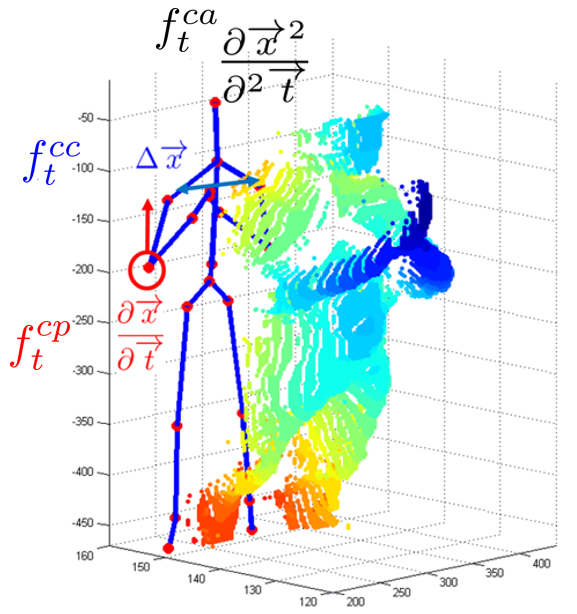
\includegraphics[width=0.3\textwidth]{images/point_cloud}\\
  \caption{
    A point cloud projection of a depth image and the 3D positional features.}
    \label{point_cloud}
\end{figure}


\subsubsection{Skeleton input features}

Given our task, only  the $\numberofjoints=11$ upper body joints are relevant and 
considered, namely \emph{``ElbowLeft, WristLeft, ShoulderLeft, HandLeft, ElbowRight, WristRight, ShoulderRight, HandRight, Head, Spine, HipCenter"}.
%
The raw skeleton features of time $t$ are defined as $\skrawfeature_t=[\framefeature_t^{s,1}, \ldots, \framefeature_t^{s, \numberofjoints}]$. 
To capture the gesture dynamics, rather than using $\skrawfeature_t$ as raw input to our data driven approach, 
we follow the approach of~\cite{diwucvpr14} and compute the 3D positional pairwise differences of joints as well as temporal derivatives, defined as (as shown in Fig.~\ref{point_cloud}) \footnote{Note that the offset features used in~\cite{diwucvpr14} depend on the first frame.
Thus if the initialisation fails which is a very common scenario, the feature descriptor will be generally very noisy. 
Hence, here we do not use these offset features.}:
\begin{align}
f^{cc}_t&=\{x_t^{s,i}-x_t^{s,j} | i,j=1,2,\ldots, N_j; i\neq j\} \label{sk_features_1}\\
f^{cp}_t&=\{x_{t+1}^{s,i}-x_t^{s,i} |  i=1,2,\ldots, N_j\} \label{sk_features_2}\\
f^{ca}_t&=\{x_{t+1}^{s,i} - 2 \times x_t^{s,i} + x_t^{s,i} | i=1,2,\ldots, N_j  \} \label{sk_features_3}
\end{align}
%
This results in an input feature vector $f_t=[f^{cc}_t, f^{cp}_t, f^{ca}_t]$ of dimension $N_f=N_j \times( \frac{ N_j}{2} + N_j + N_j)*\mathit{3}=891$.
Admittedly, here we do not completely neglect human prior knowledge about information extraction for relevant static postures, velocity and acceleration of overall dynamics of motion data.
While we have indeed used prior knowledge to define our relevant features, we believe they remain quite general and do not need dataset specific tuning.
Note that the feature extraction process resembles the computation of the 
\emph{Mel Frequency Cepstral Coefficients (MFCCs)} and their temporal derivatives 
typically used in the  speech recognition community~\cite{mohamed2012acoustic}.
%\textbf{\emph{Caveat}}:
%\begin{itemize}
%\item  When extracting skeletal features, the 3D joint coordinates have not been transformed from the world coordinate system to a person centric coordinate system by placing the \emph{``HipCenter"} at the origin.
%\item  Note also that the normalization scheme by scaling the skeleton position using length of \emph{``HipCenter"} and \emph{``Spine"} didn't work well in the implementation.
%\item The third point worth noting is that some actors performed gestures using left hand as a dominant hand whereas some using right hand which worth investigating the effect of this in the future. However, those tokens are treated indiscriminately.  Hence, the feature fed into \emph{GRBM} are almost raw, un-preprocessed.
%\end{itemize}

\subsubsection{Modeling \randomvariableSK{} using Deep Belief Networks}


%We briefly introduce the building elements of the network and a more detailed introduction can be found at:
%Boltzmann Machines (BMs) are a special structure of Markov Random Field (MRF), \emph{i.e.} the energy function is linear in term of its corresponding free parameters.
%To empower the expressiveness of the model so as to encode complex distributions, the hidden variables are introduced to enhance the modelling capability of the Boltzmann Machines

%Restricted Boltzmann Machines (RBMs) is a subtype of BMs in that there is no connections between visible to visible or hidden to hidden variables. RBM, as a special type of Markov random field with a two-layer structure, has the visible binary stochastic units $v\in \{0,1\}^D$ connected to the hidden binary stochastic units $h\in \{0,1\}^F$.
%
%The energy of the state $\{v,h\}$is:
%\begin{eqnarray}
%E(v,h;\theta)&=&-v ^{\top}Wh-b^{\top}v-a^{\top}h  \\
%             &=&-\sum^D_{i=1} \sum^F_{j=1} W_{ij} v_i h_j -\sum^D_{i=1}b_iv_i - \sum^F_{j=1}a_jh_j
%   \label{energy}
%\end{eqnarray}
%where $\theta=\{W,b,a\}$ are the free parameters: $W_{i,j}$ serves as the symmetric synergy term between visible unit $i$ and hidden unit $j$; $b_i$ is the bias term of the visible units and $a_j$ is the bias term of the hidden units.
%The joint distribution over the visible and hidden units is defined by:
%\begin{eqnarray}
%    P(v,h;\theta)&=&\frac{1}{Z(\theta)} \exp(-E(v,h;\theta)); \\
%        Z(\theta)&=&\sum_v \sum_h exp(-E(v,h;\theta))
%    \label{RBM}
%\end{eqnarray}
%The conditional distributions needed for inference and generation are given by:
%\begin{eqnarray}
%    P(h_{j=1}|\textbf{v})&=&g(\sum_i W_{ij}v_i+a_j)); \\
%      P(v_{i=1}|\textbf{h})&=&g(\sum_j W_{ij}h_j+b_i))
%\end{eqnarray}
%where $g(x)=\frac{1}{1+exp(-x)}$ is the logistic function.

%The derivative of the log-likelihood with respect to the model parameter from Eq.~\ref{RBM} is expressed as: $E_{P_{data}}[vh^{\top}]-E_{P_{model}}[vh^{\top}]$ where $E$ denotes the expectation.
%Due to the intractability of the second term, an approximation is generally required. This approximation is called the ``Constrative Divergence":
%%In practice, learning is done by following an approximation to the gradient of a different objective function, called the ``Constrative Divergence":
%\begin{equation}
%    \Delta W = \alpha (E_{P_{data}}  [\textbf{vh}^T]-E_{P_T}[\textbf{vh}^T]). \label{CD1}
%\end{equation}
%where $\alpha$ is the learning rate and $P_T$ is the distribution obtained by running a Gibbs chain, initialized with the visible units given by the data, for $T$ full steps.
Once we have the skeleton input feature \skfeature{} which served as the input \randomvariableSK{} for DBN in Fig.~\ref{GM}. The emission probability \emissionprob{} can be generated using a Deep Belief Networks.
Because input skeletal features \skfeature{} are continuous instead of binomial features, we use the Gaussian-Bernoulli RBM (\emph{GRBM})~\cite{salakhutdinov2009learning} to model the energy term of first layer with continuous visible units $v$ of dimension $D$ connected to the hidden binary stochastic units $h\in \{0,1\}^F$. More precisely:
\begin{equation}
    E(v,h;\theta) =-\sum^D_{i=1} \frac{(v_i-b_i)^2}{2\sigma_i^2} -\sum^D_{i=1} \sum^F_{j=1} W_{ij}  h_j \frac{v_i}{\sigma_i}- \sum^F_{j=1}a_jh_j
\label{GRBMenergy}
\end{equation}
where $\theta=\{W,b,a\}$ are the free parameters: $W_{i,j}$ serves as the symmetric synergy term between visible unit $i$ and hidden unit $j$; $b_i$ is the bias term of the visible units and $a_j$ is the bias term of the hidden units.

The conditional distributions needed for inference and generation are given by:
\begin{equation}
    P(h_{j=1}|\textbf{v})=g(\sum_i W_{ij}v_i+a_j));
\end{equation}
\begin{equation}
    P(v_{i=1}|\textbf{h})=\mathscr{N}(v_i|\mu_i,\sigma_i^2).
\end{equation}
where $\mu_i=b_i+\sigma_i^2 \sum_j W_{ij} h_j$ and $\mathscr{N}$ is the normal distribution. In general, we normalise the data (mean substraction and standard deviation division) in the preprocessing phase. Hence, in practice, instead of learning $\sigma_i^2$, one would typically use a fixed, predetermined unit value $\textbf{\emph{1}}$ for $\sigma_i^2$.

\begin{figure}[t]
  \centering
  % Requires \usepackage{graphicx}
  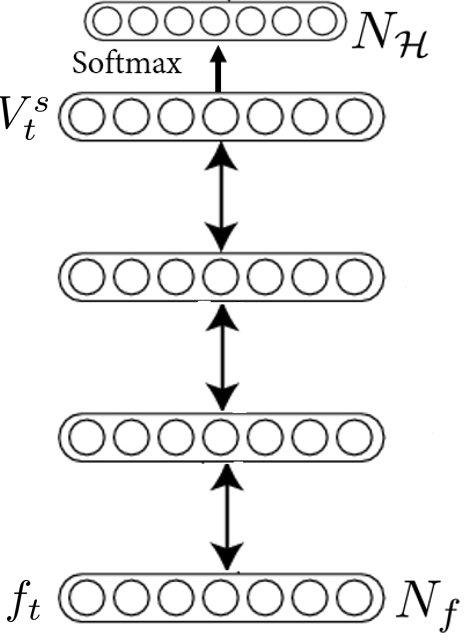
\includegraphics[width=0.23\textwidth]{images/DBN}\\
  \caption{
    Deep Belief Network using skeleton input \skfeature{} to predict emission probability \emissionprob{}.}
    \label{DBN}
\end{figure}

By stacking a softmax layer on top of the RBMs as in Fig.~\ref{DBN}, a Deep Belief Network is built for predicting emission probability \emissionprob{}. The weights are fine-tuned slightly from the top.

For high-level skeleton feature extraction, the network architectures is $[N_f,2000,2000,1000,N_{\mathcal{H}}]$,
 where $N_f = 891$ is the observation domain dimensionality; $N_{\mathcal{H}}$ is the output target class.






 In the training set, there are in total $400\,117$ frames. During the training of the \emph{DBN}, $90\%$ is used for training, $8\%$ for validation (for the purpose of early stopping) $2\%$ is used for test evaluation.
The feed forward networks are pre-trained with a fixed recipe using stochastic gradient decent with a mini-batch size of 200 training cases. Unsupervised initialisations (we run 100 epochs for unsupervised pre-training) tend to avoid suboptimal local minima and increase the network’s performance stability. For Gaussian-Bernoulli RBMs, the learning rate is fixed at 0.001 while for binary-binary RBMs the learning is 0.01 (note that in general, training \emph{GRBMs} requires smaller learning rates). For fine-tuning, the learning rate starts at 1 with 0.99999 mini-batch scaling. During the experiments, early stopping occurs around epoch 440.
The optimisation completes with a frame based validation error rate of $16.5\%$, with $16.15\%$ on the test set. The frame based validation error rate is shown in Fig~\ref{sk_error_rate} .

% Although that further optimising the network architecture would lead to more competitive results, in order not to overfit, ``as algorithms over time become too adapted to the data set, essentially memorising all its idiosyncrasies, and losing ability to generalise"~\cite{torralba2011unbiased}, we would like to treat the model as the aforementioned more generic approach.
% Since a completely new approach will initially have a hard time competing against established, carefully fine-tuned methods.
%More fundamentally, it may be that the right way to treat dataset performance numbers is not as a competition for the top place.
%This way, fundamentally new approaches will not be forced to compete for top performance right away, but will have a chance to develop and mature.
The performance of the skeleton module is shown in Tab.~\ref{Table_score_fusion}.

\begin{figure}[t]
  \centering
  % Requires \usepackage{graphicx}
  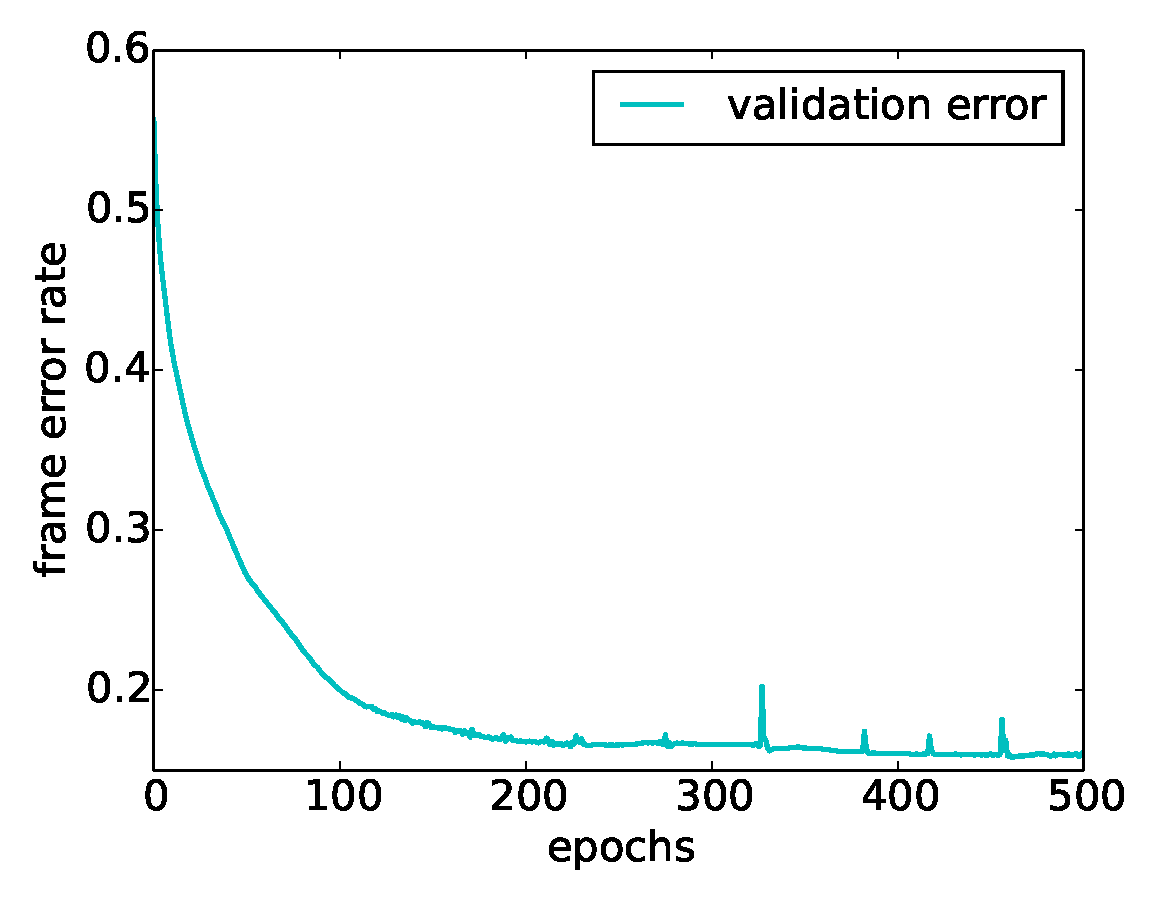
\includegraphics[width=0.4\textwidth]{images/training_error_sk}\\
  \caption{
    Deep belief network frame based validation error rate for the skeleton input module. The 0.05 frame error rate indicates the well generalisation Deep Belief Network of skeleton modules.}
    \label{sk_error_rate}
\end{figure}

\subsection{RGB \& Depth 3D Module} \label{sec:rgbd_modules}
\subsubsection{Preprocessing}\label{3d_preproc}

Although DeepMind technology~\cite{mnih2013playing} presented the first deep learning model to successfully learn control policies directly from high-dimensional sensory input using deep reinforcement learning, working directly with raw input Kinect recorded data frames, which are $640 \times 480$ pixel images, can be computationally demanding.
Therefore, our first step in the preprocessing stage consists of cropping the highest hand and the upper body using the given joint information. In the Chalearn dataset, we determined that the highest hand is the most interesting. When both hands are used, they normally perform the same (mirrored) movement, and when one hand is used, it is always the highest one which is relevant.
Furthermore, to be invariant to handiness, we train the model with the right hand view. That is, when the left hand is actually the performing hand, the video was mirrored.


The preprocessing results in four video samples (body and hand with grayscale and depth) of resolution $64\times64$. Furthermore, the noise in the depth maps is reduced by thresholding, background removal using the user index, and median filtering.
The depth images are normalised with mean substraction for each image because the median of depth images are irrelevant to the gesture subclass. And both RGB and depth images are normalised by dividing the standard deviation of each image.
The outcome is illustrated in Fig.~\ref{3dcnn_filters} (left).
%\begin{figure}[t]
%  \centering
%  % Requires \usepackage{graphicx}
%  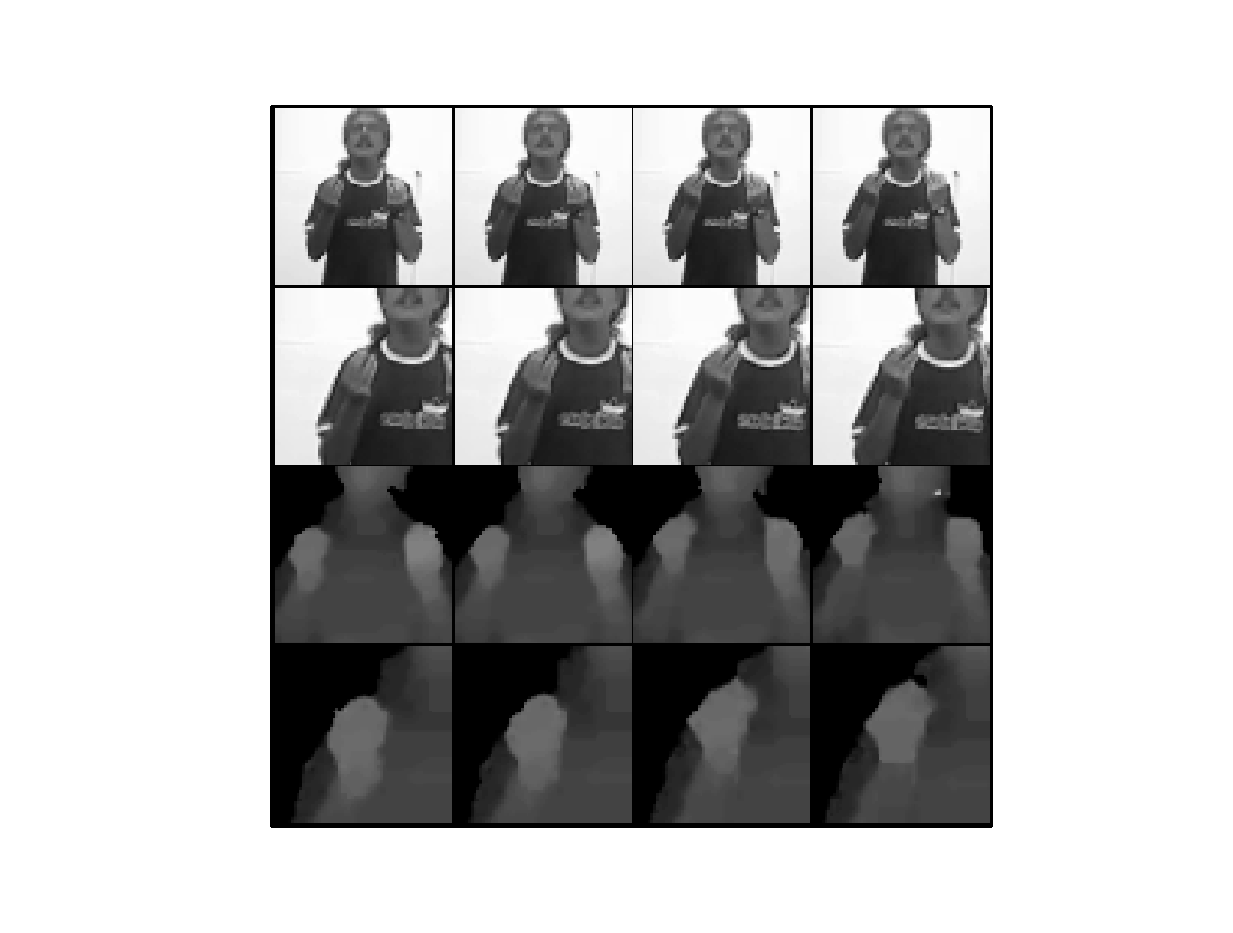
\includegraphics[width=0.5\textwidth]{images/3dcnn_filters/original.eps}\\
%  \caption{
%    Preprocessing result. Inputs  from top to bottom: 1) grayscale body input, 2) grayscale hand input, 3) depth body input, 4) depth hand input. }
%    \label{3dcnn input}
%\end{figure}


\subsubsection{3DCNN Architecture}
\begin{figure*}[t]
  \centering
  % Requires \usepackage{graphicx}
  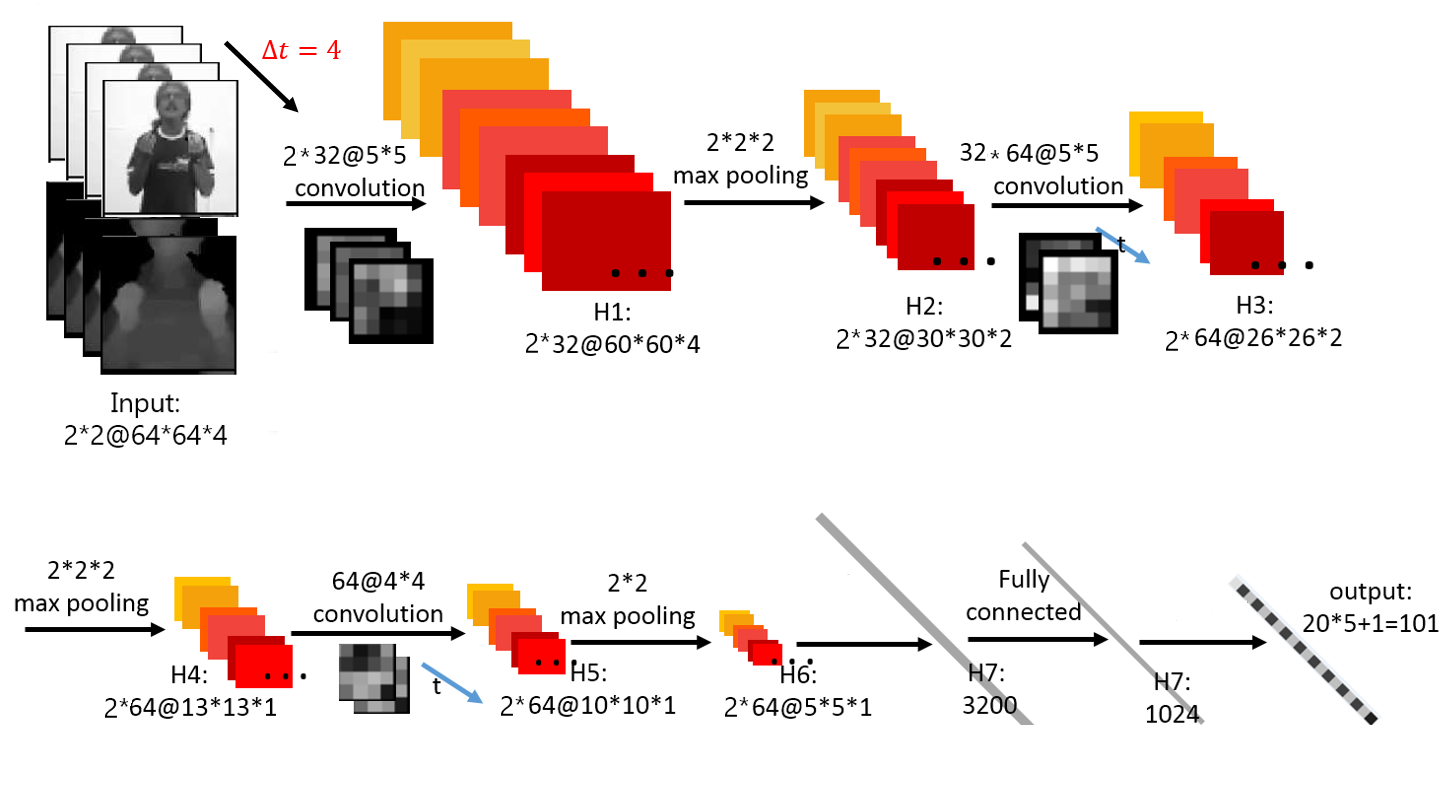
\includegraphics[width=.9\textwidth]{images/3DCNN_new}
  \caption{An illustration of the architecture of the 3DCNN architecture. The 3rd dimension of the input is time with 4 frames stacked together. The depth and RGB data are stacked (concatenated) together at Input. Hand and body part output are concatenated at H7.}\label{3dcnn_architecture}
\end{figure*}

This deep neural network architecture consists of a series of layers composed of either convolution, pooling or, in the last layer, fully connected layers.
The 3D convolution itself is achieved by convolving a 3D kernel to the cuboid formed by stacking multiple contiguous frames together. We follow the nomenclature as in~\cite{ji20133d}.
 However, instead of using $tanh$ units as in~\cite{ji20133d},  Rectified Linear Units (\emph{ReLUs})~\cite{krizhevsky2012imagenet} were used in order to speed up training.
 Formally, the value of a unit at position $(x, y, z)$ ($z$ here corresponds to the time-axis) in the $j$-th feature map in the $i$-th layer, denoted as $v^{xyz}_{ij}$, is given by:
\begin{equation}
v^{xyz}_{ij} =  max( 0,  ( b_{ij} + \sum_m \sum_{p=0}^{P_i - 1} \sum_{q=0}^{Q_i -1 } \sum_{r=0}^{R_i -1} w^{pqr}_{ijm} v^{(x+p)(y+q)(t+r)}_{(i-1)m} ))
\label{ReLU}
\end{equation}

The complete 3DCNN architecture is depicted in Fig.~\ref{3dcnn_architecture} : 4 types~(Fig.~\ref{3dcnn_filters}) of input contextual frames are stacked as size $64\times64\times4$.
The first layer consists of 32 feature maps produced by $5\times5$ spatial convolutional kernels followed by local contrast normalisation (LCN)~\cite{jarrett2009best} and 3D max pooling with strides $(2,2,2)$, then the grayscale channel and depth channel are concatenated. The second layer has 64 feature maps with $5\times5$ kernels followed by LCN and 3D max pooling with strides $(2,2,2)$. The third layer is composed of 64 feature maps with $4\times4$ kernels followed by 3D max pooling with strides $(1,2,2)$. All convolutional layer outputs are flattened with the body channel and hand channel concatenated, and fed into one fully connected layer of size $1024$. The output layer has \numberhiddenstates{} values, the number of states in the HMM in Fig.~\ref{HMM_ES}.




\subsubsection{Details of Learning}
% The first 650 batches are used for training and the remaining 50 files for validation.
During training, dropout \cite{hinton2012improving} is used as main regularisation approach to reduce overfitting. Nesterov’s accelerated gradient descent (NAG) \cite{sutskever2013importance} with a fixed momentum-coefficient of 0.9 and mini-batches of size 64 are also used.
The learning rate is initialised at 0.003 with a 5\% decrease after each epoch. The weights of the 3DCNNs are randomly initialised with a normal distribution with $\mu = 0$ and $\sigma = 0.04$.
The frame based validation error rate is $39.06\%$ after 40 epochs as shown in Fig.~\ref{error rate}. Compared with the skeleton module (16.5\% validation error rate), the 3DCNN has a notable higher frame based error rate.


\begin{figure}[t]
  \centering
  % Requires \usepackage{graphicx}
  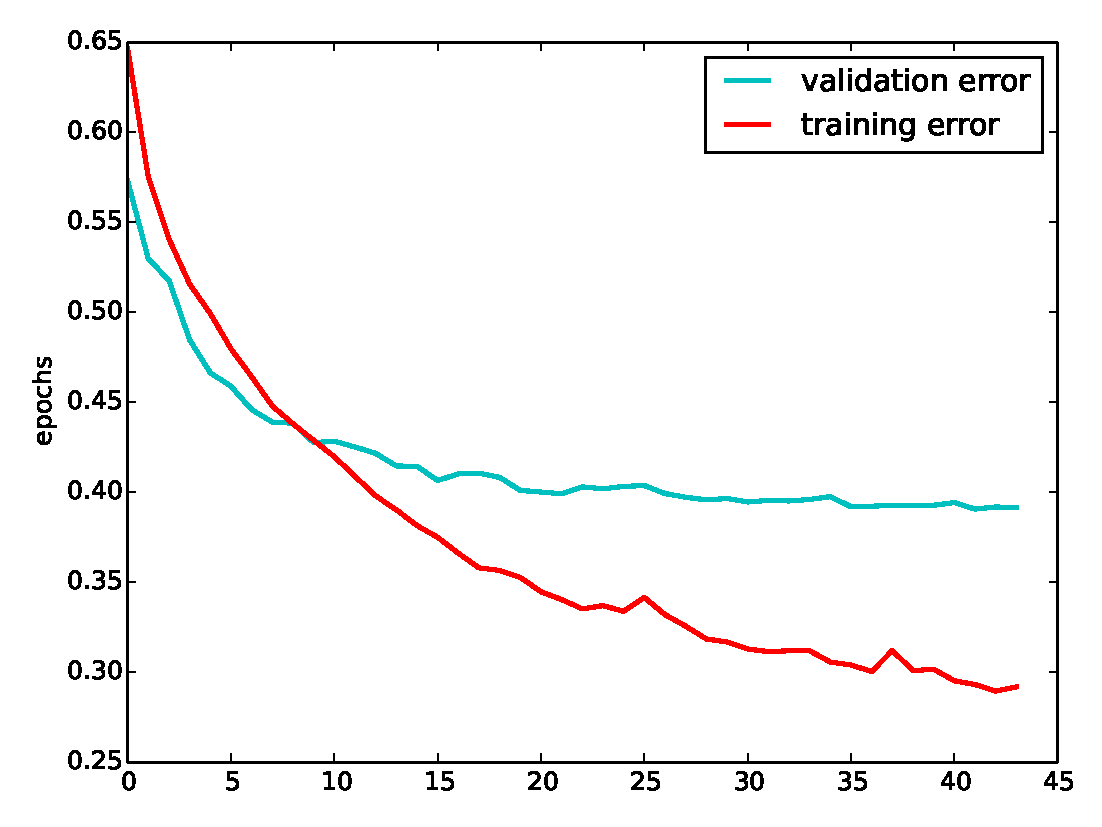
\includegraphics[width=.4\textwidth]{images/3dcnn_filters/training_error}
  \caption{The frame based error rate for training 3DCNN. The frame error rates from 3DCNN are much higher than the skeleton module in~\ref{sk_error_rate} which indicates learning from images may be more difficult than from skeleton modules. }\label{error rate}
\end{figure}

\subsubsection{Looking into the Networks: visualisation of Filter Banks}

The convolutional filter weights of the first layer are depicted in Fig.~\ref{3dcnn_filters}. The unique characteristics from the kernels are clearly visible: as hand inputs have larger homogenous areas than the body inputs, hence the hand part filters are smoother than their body counterpart.
In addition, depth images have sharper edges as also observed in~\cite{socher2012convolutional} and while being smooth overall than the grayscale filters.

\begin{figure*}[t]
  \centering
  % Requires \usepackage{graphicx}
  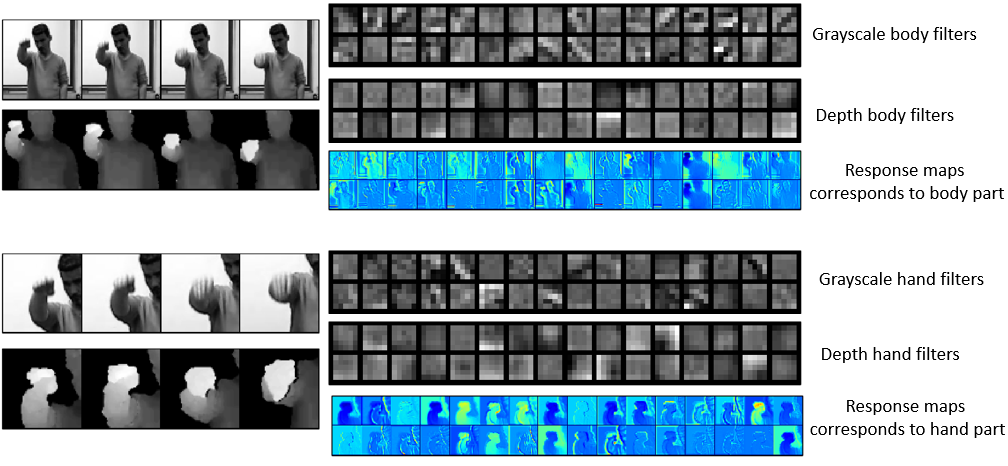
\includegraphics[width=0.85\textwidth]{images/CNN_filters}
  \caption{Visualisation of input frames, first convolutional layer $5\times5$ filters and the corresponding response maps for body and hand parts. Because depth channel is smoother than the RGB grayscale channel, the corresponding filter maps are smoother as well. }\label{3dcnn_filters}
\end{figure*}


\subsection{Multimodal Fusion}
To combine the two modalities, two strategies can be used, as shown in Fig.~\ref{fig:fusion}: a late fusion approach and an early fusion approach.


\subsubsection{Late Fusion}
Formally, this multimodal fusion scheme corresponds to the fusion of the emission probabilities estimated from the different input. While different schemes exits, a simple linear combination:

\begin{equation}
\emissionprob  \propto  \alpha \cdot \emissionprobSK + (1-\alpha)\cdot \emissionprobRGBD
\end{equation}
where different emission probabilities are provided by the modules described in \ref{sec:skeleton_module} and \ref{sec:rgbd_modules} and $\alpha$ is a coefficient that controls the contributions of each source of information estimated by cross validation.
Interestingly, the best performing $\alpha$ is close to $0.5$, indicating that both approaches are equally important.


\subsubsection{Early Fusion}\label{early_fusion}

Instead of traditional late fusion, we adopt another layer of perceptron (with 2024 hidden unites) for cross modality learning taking the input from each individual net's penultimate layer.
The parameters of two neural networks (for skeleton and depth) are loaded from the previously trained individual module. We argue that this ``pre-trained" parameters are important because the heterogenous inputs of the system.  We fine-tune the network and stop the training when the validation error rate stops decreasing ($\sim$15 epochs).

\begin{figure}[t]
  \centering
  % Requires \usepackage{graphicx}
  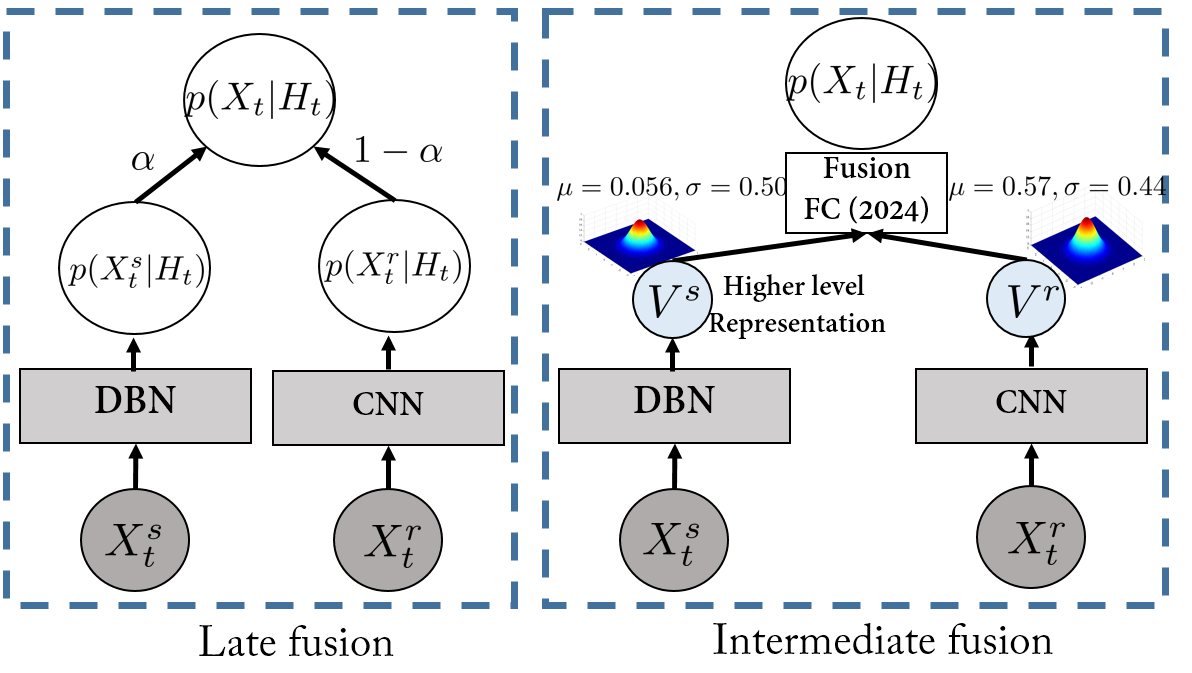
\includegraphics[width=0.5\textwidth]{images/Fusion_combined}
  \caption{
    Architecture of the multimodal dynamic networks with late fusion scheme (left) and early fusion scheme (right).  Late fusion scheme combines the emission probabilities from two modalities. For early fusion scheme, each modality (skeleton and RGB-D) is first pre-trained by a Deep Neural Network, and their penultimate layers are fused together to generate a shared representation for dual modalities. The outputs are the emission probabilities \emissionprob for temporal dynamic modeling. The Gaussians represent activations of the neurons for each input modality and the final fusion layer. The mean activation of skeleton module neurons is predominantly larger than the RGBD ConvNet's (0.57 \emph{vs.} 0.056). Note that skeleton module has logistic units whereas ConvNet module has relu unit~\cite{DBLP:journals/corr/PigouODHD15}, hence the mean activations of the two are not directly comparable. However, 10 times the difference of mean activation indicates the bias during the multimodal fine-tuning phase that could cause the less than expected performance.
  }\label{fig:fusion}
\end{figure}



\endinput
